\chapter{Graph-Datenbanken im praktischen Einsatz: OLAP}
\section{PostgreSQL: OLAP}
\subsection{Benchmark}
Mit der Standardinstallation von PostgreSQL wird auch pgbench mitinstalliert. Bei pgbench handelt es sich um ein einfaches Tool zur Durchführung von Benchmark-Tests. Bei einem Benchmark-Test wird eine Menge von \ac{SQL}-Statements beliebig oft wiederholt, dabei können auch mehrere parallele Sessions geöffnet werden. Beim durchführen des Tests berechnet pgbench die Anzahl der Transaktionen pro Sekunde.
\subsubsection{Verwendung von pgbench}
pgbench wird über die Kommandozeile gestartet. Dabei können eine Reihe von Parametern übergeben werden, mit denen das Verhalten von pgbench gesteuert werden kann.
\begin{itemize}
	\item -c clients  \\
	Über das Flag -c wird die Anzahl der Clients bzw. die Anzahl der gleichzeitigen Datenbankverbindungen festgelegt. Wenn hier nichts angegeben ist wird nur ein Client verewendet.
	\item -t transactions \\
	Über das Flag -t wird festgelegt wieviele Transaktionen jeder Client durchführt. Die Anzahl aller Transaktionen ergibt sich durch das Produkt von Clients und Transactions.
\end{itemize}
\begin{figure}[H]
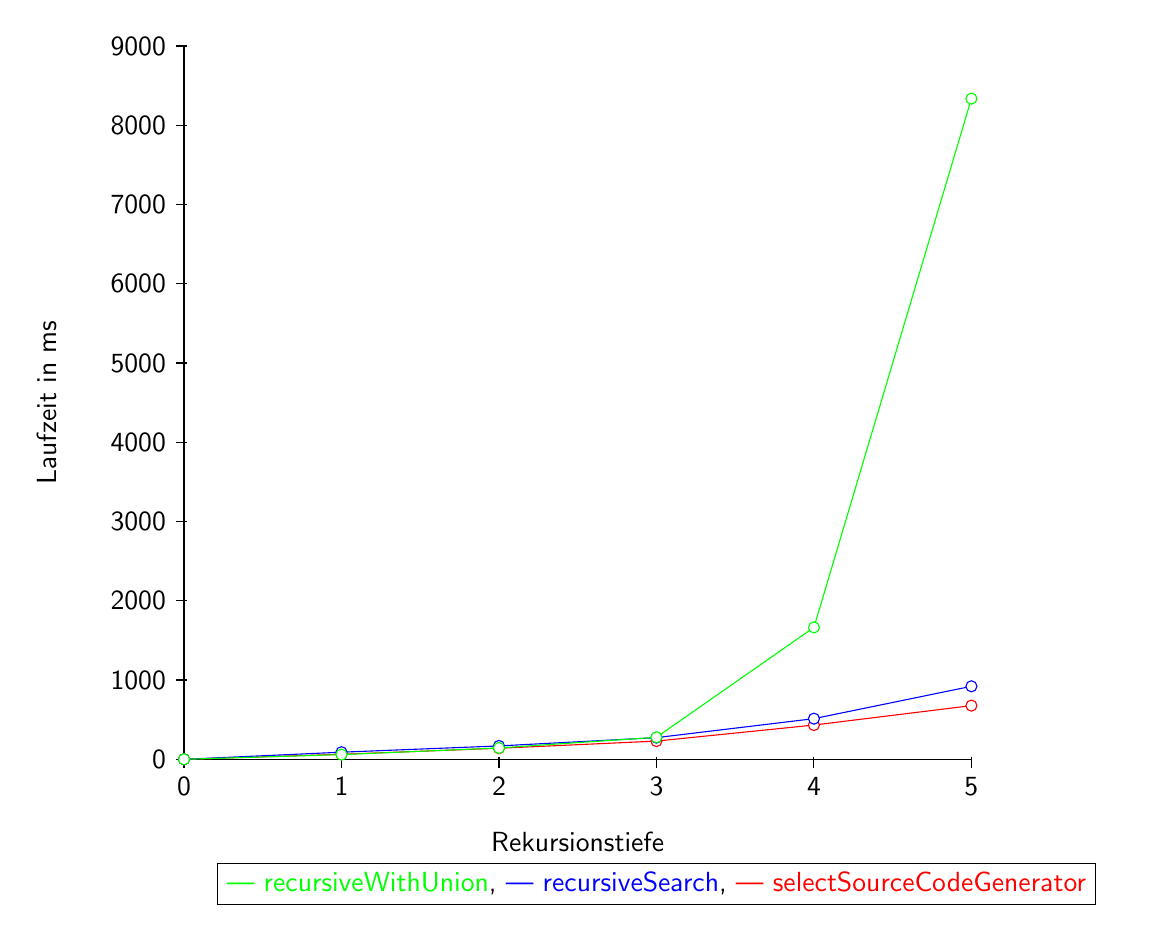
\begin{tikzpicture}[y=.001cm, x=2cm,font=\sffamily]
%axis
\draw (0,0) -- coordinate (x axis mid) (5,0);
\draw (0,0) -- coordinate (y axis mid) (0,9000);
    	%ticks
\foreach \x in {0,...,5}
\draw (\x,1pt) -- (\x,-3pt)
node[anchor=north] {\x};
\foreach \y in {0,1000,...,9000}
\draw (1pt,\y) -- (-3pt,\y)
node[anchor=east] {\y}; 
%labels      
\node[below=0.8cm] at (x axis mid) {Rekursionstiefe};
\node[rotate=90, above=1.5cm] at (y axis mid) {Laufzeit in ms};
%plots
\draw[red] plot[ mark=*, mark options={fill=white}] 
coordinates{(0, 0)
			(1, 63.636)
			(2,139.225)
			(3,229.997)
			(4,432.297)
			(5,677.420)
		};
\draw[blue] plot[ mark=*, mark options={fill=white}] 
coordinates{(0, 0)
	(1, 89.858)
	(2,168.822)
	(3,273.452)
	(4,513.038)
	(5,921.228)
};
\draw[green] plot[ mark=*, mark options={fill=white}] 
coordinates{(0, 0)
	(1, 59.275)
	(2,143.367)
	(3,277.766)
	(4,1664.168)
	(5,8335.513)
};
\draw[draw=none] (0,0) -- (6,0) node[draw, midway, yshift=-4.5em] {\textcolor{green}{--- recursiveWithUnion},
	\textcolor{blue}{--- recursiveSearch}, 
	\textcolor{red}{--- selectSourceCodeGenerator}};
\end{tikzpicture}
	\caption{ public\_epinions}
\end{figure}


\begin{table}[H]
	\centering
	\begin{tabular}{l|l|l|l|}
		\cline{2-4}
		& \multicolumn{3}{l|}{Laufzeit in MS} \\ \hline
		\multicolumn{1}{|l|}{Rerkusionstiefe} & selectSourceCodeGenerator  & recursiveSearch  & recursiveWithUnion    \\ \hline
		\multicolumn{1}{|l|}{1}               & 63.636           & 	89.858  & 59.275    \\ \hline
		\multicolumn{1}{|l|}{2}               & 139.225          & 	168.822 & 143.367   \\ \hline
		\multicolumn{1}{|l|}{3}               & 229.997          & 273.452   &  277.766   \\ \hline
		\multicolumn{1}{|l|}{4}               & 432.297          & 513.038     & 1664.168     \\ \hline
		\multicolumn{1}{|l|}{5}               & 677.420          &  921.228   & 8335.513     \\ \hline
	\end{tabular}
\end{table}
\begin{figure}[H]
	
	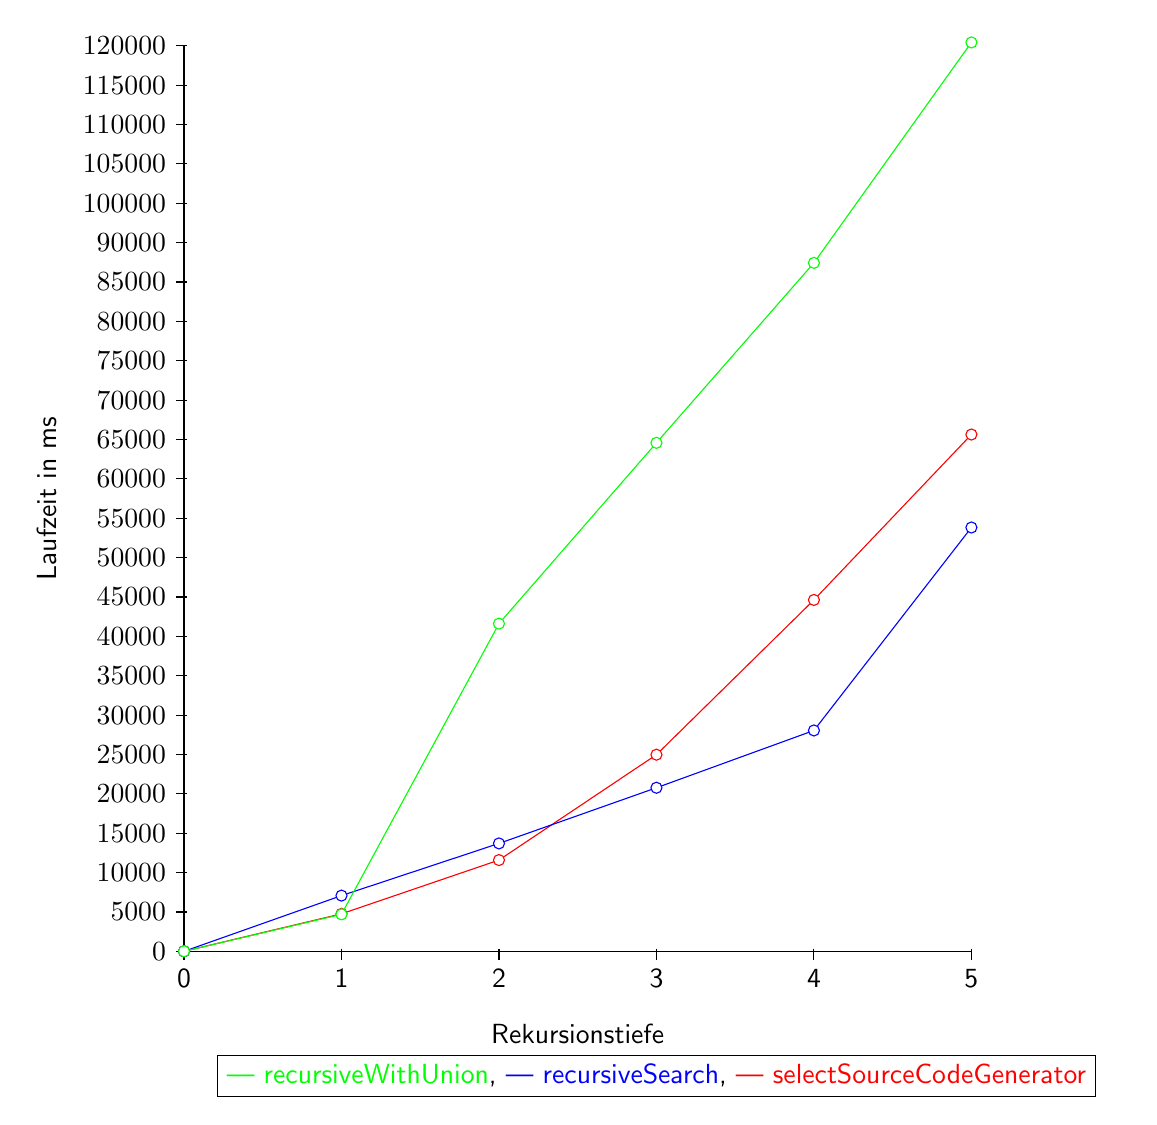
\begin{tikzpicture}[y=.5cm, x=2cm,font=\sffamily]
	%axis
	\draw (0,0) -- coordinate (x axis mid) (5,0);
	\draw (0,0) -- coordinate (y axis mid) (0,23);
	%ticks
	\foreach \x in {0,...,5}
	\draw (\x,1pt) -- (\x,-3pt)
	node[anchor=north] {\x};
	\foreach \y/\ytext in {
		0/0,
		1/5000,
		2/10000,
		3/15000,
		4/20000,
		5/25000,
		6/30000,
		7/35000,
		8/40000,
		9/45000,
		10/50000,
		11/55000,
		12/60000,
		13/65000,
		14/70000,
		15/75000,
		16/80000,
		17/85000,
		18/90000,
		19/100000,
		20/105000,
		21/110000,
		22/115000,
		23/120000,
	}
	\draw (1pt,\y) -- (-3pt,\y) node[anchor=east] {$\ytext$};
	%labels      
	\node[below=0.8cm] at (x axis mid) {Rekursionstiefe};
	\node[rotate=90, above=1.5cm] at (y axis mid) {Laufzeit in ms};
	%plots
	\draw[red] plot[mark=*, mark options={fill=white}] 
	coordinates{(0, 0)
		(1, 4761.733/5000)
		(2,	11589.219/5000)
		(3, 4.9944)	%=24971/5000
		(4, 8.9252) %=44625,935÷5000
		(5,	13.1265944)%=65632,972÷5000
	};
\draw[blue] plot[mark=*, mark options={fill=white}] 
coordinates{(0, 0)
	(1, 1.4151)%7075.399/5000)
	(2,	2.7405)%13702.381/5000)
	(3, 4.1548)%20773.827/5000)
	(4, 5.6098)%28048.866/5000)
	(5,	10.7651)%53825.401/5000)
};
\draw[green] plot[mark=*, mark options={fill=white}] 
coordinates{(0, 0)
	(1, 0.939)%4695.466/5000)
	(2,	8.323)%41616.216/5000)
	(3, 12.916)%64577.873/5000)
	(4, 17.487)%87434.075/5000)	
	(5,	23.086)%115432.071/5000)	
};
\draw[draw=none] (0,0) -- (6,0) node[draw, midway, yshift=-4.5em] {\textcolor{green}{--- recursiveWithUnion},
	\textcolor{blue}{--- recursiveSearch}, 
	\textcolor{red}{--- selectSourceCodeGenerator}};
	\end{tikzpicture}
	\caption{ public\_livejournal}
\end{figure}

\begin{figure}[H]
	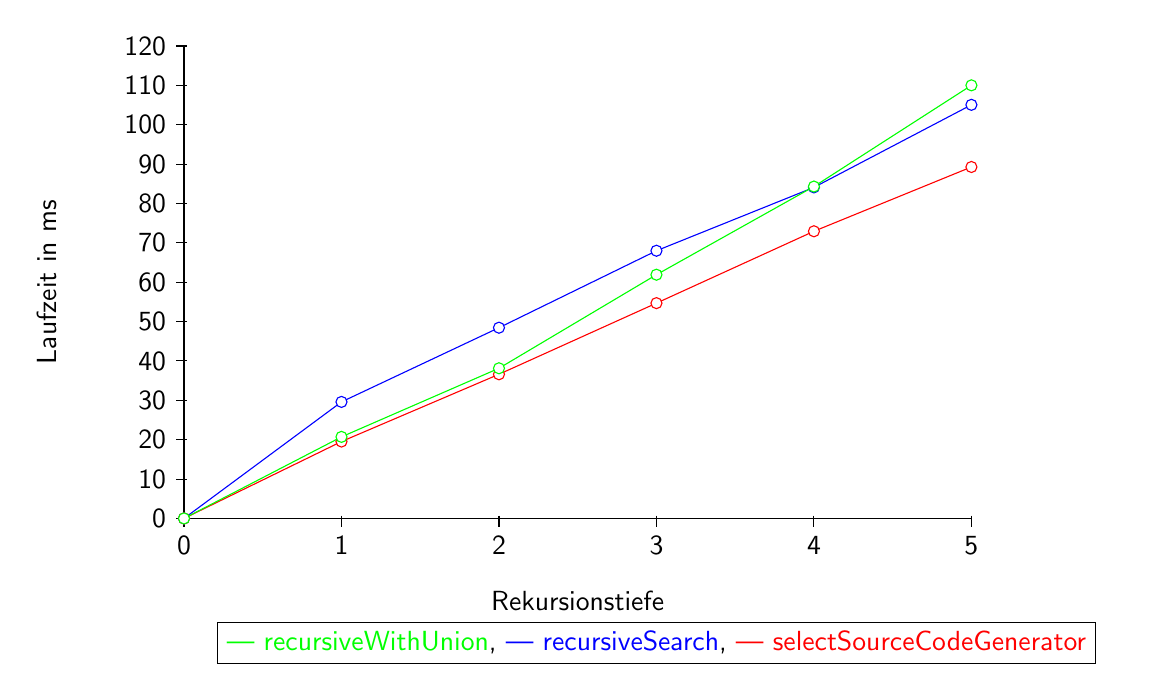
\begin{tikzpicture}[y=.05cm, x=2cm,font=\sffamily]
	%axis
	\draw (0,0) -- coordinate (x axis mid) (5,0);
	\draw (0,0) -- coordinate (y axis mid) (0,120);
	%ticks
	\foreach \x in {0,...,5}
	\draw (\x,1pt) -- (\x,-3pt)
	node[anchor=north] {\x};
	\foreach \y in {0,10,...,120}
	\draw (1pt,\y) -- (-3pt,\y)
	node[anchor=east] {\y}; 
	%labels      
	\node[below=0.8cm] at (x axis mid) {Rekursionstiefe};
	\node[rotate=90, above=1.5cm] at (y axis mid) {Laufzeit in ms};
	%plots
	\draw[blue] plot[ mark=*, mark options={fill=white}] 
	coordinates{(0, 0)
		(1, 29.595)
		(2,48.442)
		(3,67.989)
		(4,84.084)
		(5,105.049)
	};
	\draw[red] plot[ mark=*, mark options={fill=white}] 
	coordinates{(0, 0)
		(1, 19.528)
		(2,36.613)
		(3,54.681)
		(4,72.934)
		(5,89.262)
	};
	\draw[green] plot[ mark=*, mark options={fill=white}] 
	coordinates{(0, 0)
		(1, 20.716)
		(2,38.137)
		(3,61.904)
		(4,84.295)
		(5,110.000)
	};
	\draw[draw=none] (0,0) -- (6,0) node[draw, midway, yshift=-4.5em] {\textcolor{green}{--- recursiveWithUnion},
		\textcolor{blue}{--- recursiveSearch}, 
		\textcolor{red}{--- selectSourceCodeGenerator}};
	\end{tikzpicture}
	\caption{ public\_facebook}
\end{figure}


\subsection{Standard SQL}
\subsection{Stored Procedures}
\subsection{PL/SQL-Recursion}
\subsection{Datenbankzugriffe}
\subsection{Zugriffsart Aggregation}
\subsection{Zugriffsart Traversierung}
\subsection{Interpretation der Ergebnisse}